%Organize this section according to the rules defined in the project description. 
\setlength{\parskip}{0.3cm}

The target of this part is to provide a formal model of the software to be, that can be analyzed and tested. Such study is carried out in the Alloy envinronment.  Defining all the aspects of the system is not so trivial in this case, the two services, as said are not independent. ASOS uses a subset of data collected through Data4Help in order to evaluate the user condition, such data are provided by devices registered to D4H, to just name a few.
So in order to not complicate too much the model, only the following  cases are highlighted and tested to facilitate the comprehension:
\par
\textbf{Data4Help}

\begin{itemize}[topsep=-0.1cm]
	\item A third party can access a specific user dataset, only after the same user accepts such request. 
	\item A third party is provided with an anonymous dataset (Anonymous Request) if the number of anonymous users involved in an anonymous request is at least 1000. 
	\item A user dataset is composed only with data provided by registered sensor devices
\end{itemize}

\textbf{AutomatedSOS}
\begin{itemize}
	\item If an emergency condition is detected the nearest ERM is alerted
	\item Anomaly conditions can turn into emergencies only if expressed by the user or after the prevention timeout expires. The reverse conversion is not allowed. Emergency conditions can be directly triggered by critical trigger events (criticality = true).
	\item A user can have a supervisor which is notified each time an anomaly or emergency condition is detected by the system
\end{itemize}


%\section{Alloy Code}
{\color{Blue}{\subsection{Alloy Code}}}
%\subsection{Signatures}
{\color{Blue}{\subsubsection{Signatures}}}
\lstinputlisting[language=alloy]{alloy_code/signatures.als}

%\subsection{Facts and Asserts}
{\color{Blue}{\subsection{Facts and Asserts}}}
\lstinputlisting[language=alloy]{alloy_code/facts_asserts.als}

%\subsection{Predicates}
{\color{Blue}{\subsubsection{Predicates}}}
\lstinputlisting[language=alloy]{alloy_code/predicates.als}

%\subsection{Testing}
{\color{Blue}{\subsubsection{Testing}}}
\lstinputlisting[language=alloy]{alloy_code/testing.als}

\begin{figure}[htp!]
	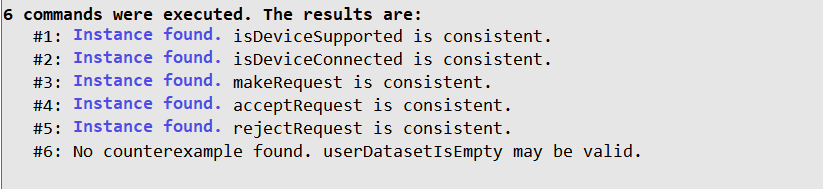
\includegraphics[scale=0.8]{Images/alloy/D4H_consistency.png}
	\captionsetup{justification=raggedright, singlelinecheck=false}
	\vspace*{-2mm}\caption{Consistency Test of D4H model}
	\label{figure17}
\end{figure}
\begin{figure}[htp!]
	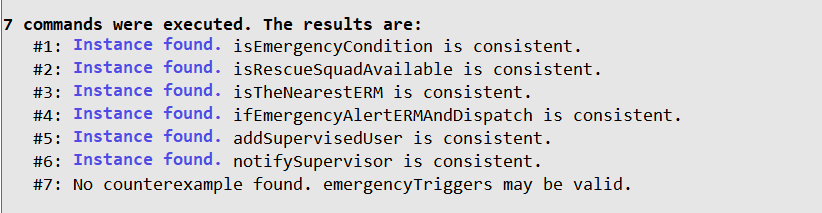
\includegraphics[scale=0.8]{Images/alloy/ASOS_consistency.png}
	\captionsetup{justification=raggedright, singlelinecheck=false}
	\vspace*{-2mm}\caption{Consistency Test of ASOS model}
	\label{figure18}
\end{figure}
\newpage
{\color{Blue}{\subsubsection{Data4Help World}}}
%\subsection{Data4Help World}
\begin{figure}[H]
	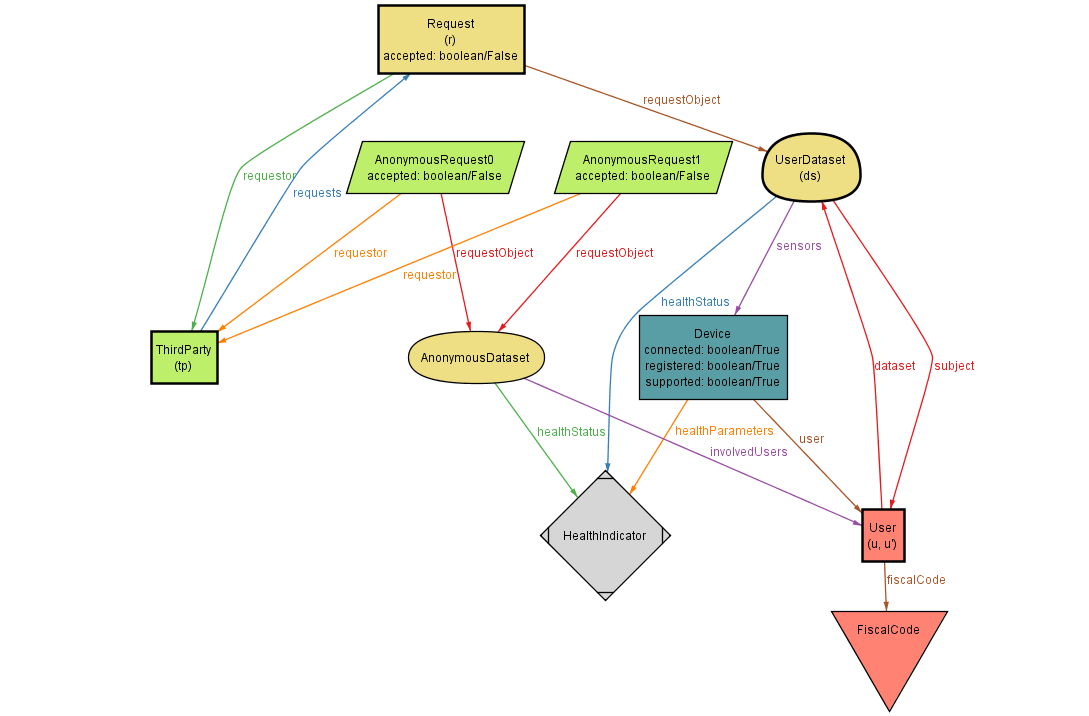
\includegraphics[scale=0.42]{Images/alloy/D4H_world.png}
	\vspace*{-3mm}\caption{Data4Help world generated after testing}
	\label{figure19}
\end{figure}


%\subsection{AutomatedSOS World}
{\color{Blue}{\subsubsection{AutomatedSOS World}}}

\begin{figure}[H]
	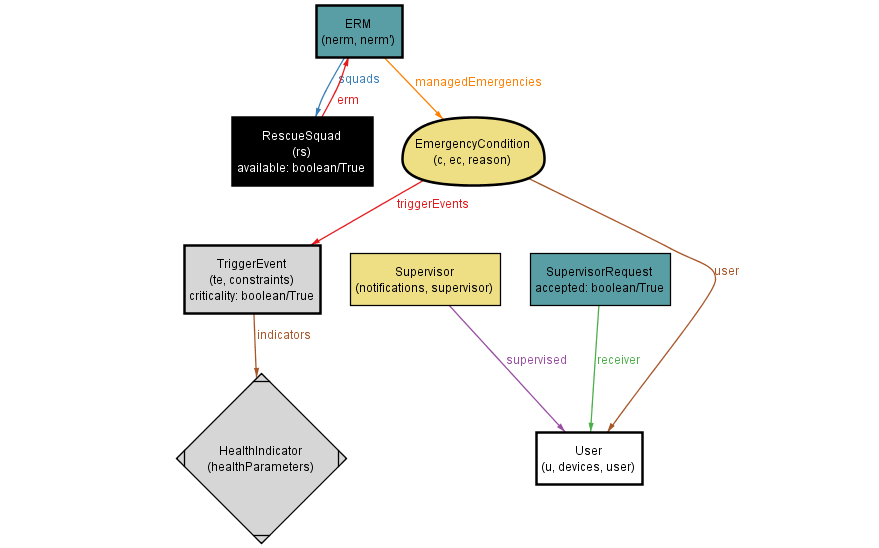
\includegraphics[scale=0.45]{Images/alloy/ASOS_world.png}
	\vspace*{-2mm}\caption{AutomatedSOS world generated after testing}
	\label{figure20}
\end{figure}








